\begin{frame}[standout]
	What if Neural Networks had SVDs?
\end{frame}

\begin{frame}{The Singular Value Decomposition}
	\begin{definition}
		The Singular Value Decomposition of $W \in \R^{m\times n}$ is a factorization
		$W = U \Sigma V^T$, where  $U$ is an \alert{orthogonal} $m \times m$ matrix,
		$\Sigma$ is an $m \times n$ rectangular diagonal matrix, and $V$ is an $n \times
		n$ \alert{orthogonal} matrix.
	\end{definition}
\end{frame}

\begin{frame}{Properties of the SVD}
	For out purposes, assume that $W$ is a square, i.e., $W \in \R^{d\times d}$.
	Then:
	\begin{align*}
		U^{-1} &= U^T\text{ and }V^{-1} = V^T  \quad \quad & O(d^2)\\
		W^{-1} &= (U \Sigma V^T)^{-1} = V \Sigma^{-1} U^T  & O(d^2)\\
		det(W) &= \prod_{i=1}^{d} \Sigma_{i,i}   & O(d)
	\end{align*}
	Other fast computations are largest singular value, condition number, matrix exponential, and Cayley Map.
\end{frame}

\begin{frame}{Use in Neural Networks}
	% Titles
	\begin{columns}
		\begin{column}{0.47\textwidth}
			\alert{Neural Networks}
		\end{column}
		\begin{column}{0.47\textwidth}
			\alert{Gradients}
		\end{column}
	\end{columns}
	\vspace{1em}

	\begin{columns}
		\begin{column}{0.47\textwidth}
			Recall a simple fully-connected layer:
			\begin{equation*}
 				h_{\ell} = \sigma (Wh_{\ell-1}) = \sigma \left( U\Sigma V^T h_{\ell-1}\right)
			\end{equation*}

			\begin{itemize}
				\item Normalizing flows
				\item Recurrent Neural Networks
				\item W-GAN
			\end{itemize}
		\end{column}

		\begin{column}{0.47\textwidth}
			% What happens when we use gradient descent?
			\begin{align*}	
				W^{t+1} &= W^{t} - \eta \frac{\partial L}{\partial W}\\
				\Sigma^{t+1} &= \Sigma^{t} - \eta \frac{\partial L}{\partial \Sigma}\\
				U^{t+1} &= U^{t} - \eta \frac{\partial L}{\partial U}\\
			\end{align*}
		\end{column}
	\end{columns}
\end{frame}

\begin{frame}{The Householder Matrix}
	\begin{definition}
 		For a vector $v \in \R^{d}$, the corresponding Householder matrix
 		is defined as
 		\begin{equation}\label{eq:hh}
 			H = I - 2\frac{v v^T}{||v||^2_2}
 		\end{equation}
	\end{definition}

	\begin{itemize}
		\item Note LHS of Eqn. (\ref{eq:hh}) takes $O(d^2)$ but RHS takes $O(d)$.
		\item $H$ stays orthogonal under gradient descent on $v$!
	\end{itemize}

	\begin{lemma}
		The product of two orthogonal matrices is orthogonal. 
	\end{lemma}
\end{frame}

\begin{frame}{Main Idea}
	Parametrize $U$ and $V$ as a product of Householder matrices \cite{orthhh}.
	
	$$
		U = H_1 \cdot H_2 \cdots H_{d}
	$$

	When evaluating a NN, we need to compute

	$$
		UX = H_1 ( H_2 ( \cdots (H_{d} X)))
	$$

	with $X \in \R^{d \times m}$, where $m$ is the batch size.

	If we represent $H_i$s as matrices, this takes $O(d^3m)$ time (denoted \myparallel~\cite{orthhh}).
	We can easily improve by representnig $H_i$ by its vectors
	$v_i$ instead, $O(d^2m)$ (denoted \mysequential~\cite{orthhh}).
	%$v_i$ instead, $O(d^2m)$ (denoted \emph{sequential}).
\end{frame}

\begin{frame}{Issues}
	
	\textbf{Issues:}
	\begin{itemize}
		\item The \myparallel~algorithm is slow in theory.
		\item The \mysequential~algorithm is not suited for GPUs.
	\end{itemize}

	\textbf{We propose:}
	\begin{itemize}
		\item Algorithm which is suited for GPUs and fast in theory.
	\end{itemize}

\end{frame}

\begin{frame}{Our Algorithm}

	\begin{lemma}
		\cite{wydec} For any $m$ Householder matrices $H_1,...,H_m$ there exists $W,Y\in \R^{d\times m}$ st. 
		$$I-2WY^T = H_1 \cdots H_m. $$
		Both $W$ and $Y$ can be computed by $m$ sequential Householder multiplications in $O(dm^2)$ time. 
	\end{lemma}

	\begin{center}
		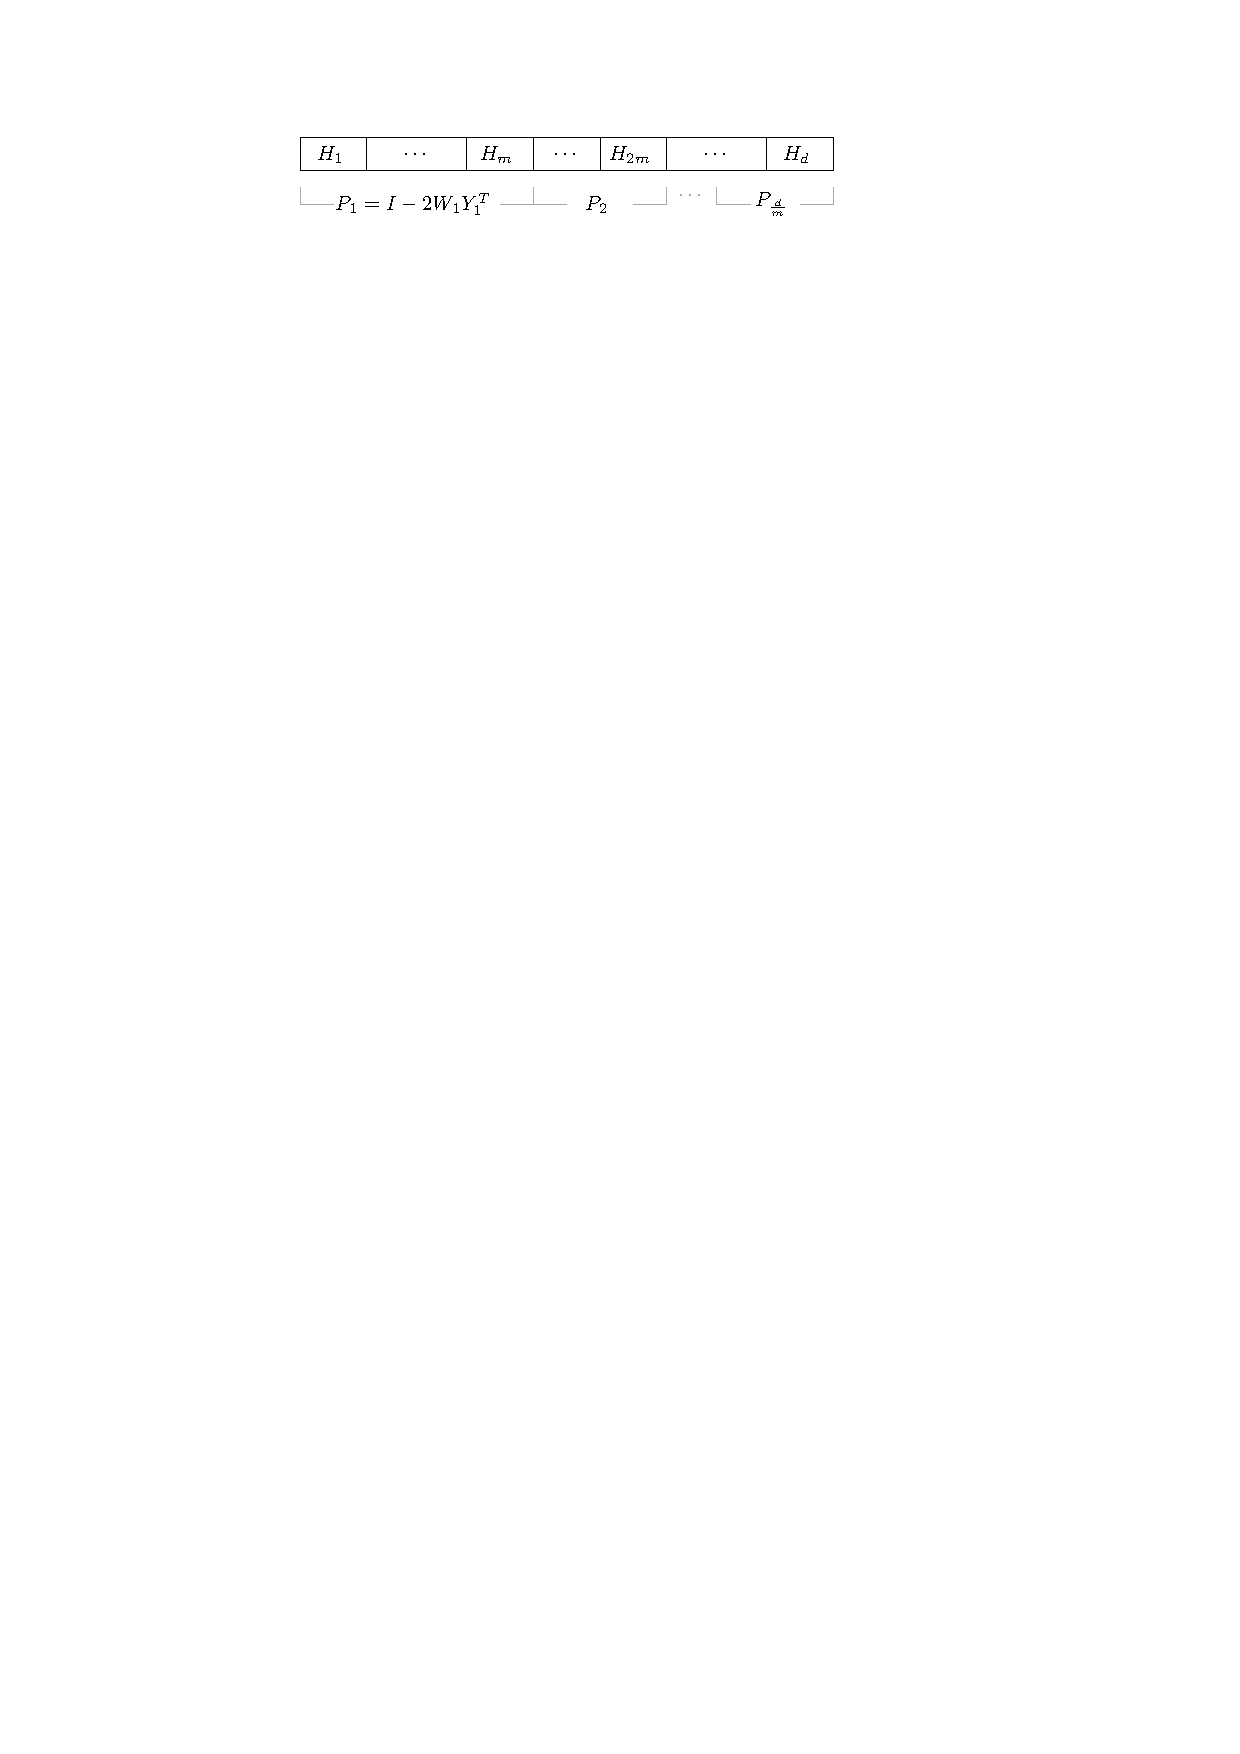
\includegraphics[width=0.7\textwidth, page=1]{graphics}
	\end{center}

\end{frame}

\begin{frame}{Complexity}

		\textbf{Time:} 
		$$P_1 \cdot P_2 \cdots P_{\frac{d}{m}} X \qquad O(d^3m) \Rightarrow O(d^2m) $$
		\textbf{\# sequential opetations:} 
		$$O(\text{compute }I-2WY^T + \text{multiply }P_i\text{s}) = O(d/m + m)$$

\end{frame}

\begin{frame}{Experiments}
	\begin{columns}
		\begin{column}{0.49\textwidth}
			\vspace{1em}
			\centering
			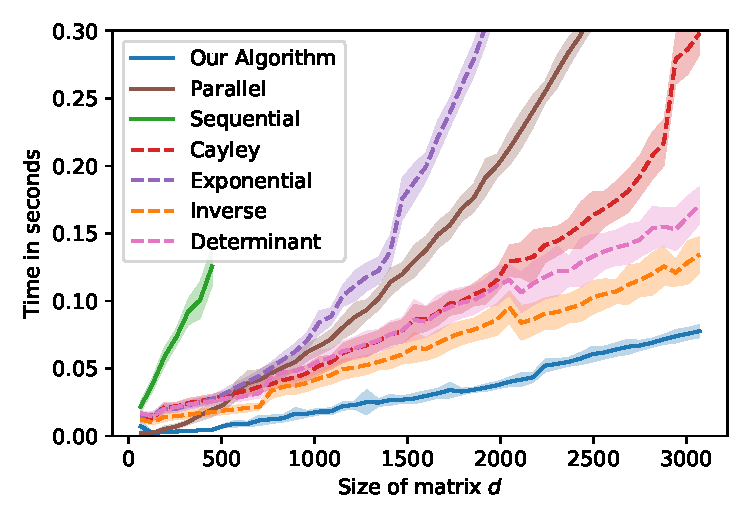
\includegraphics[width=\textwidth]{matrix_operations}
		\end{column}
		\begin{column}{0.49\textwidth}
			\vspace{1em}
			\centering
			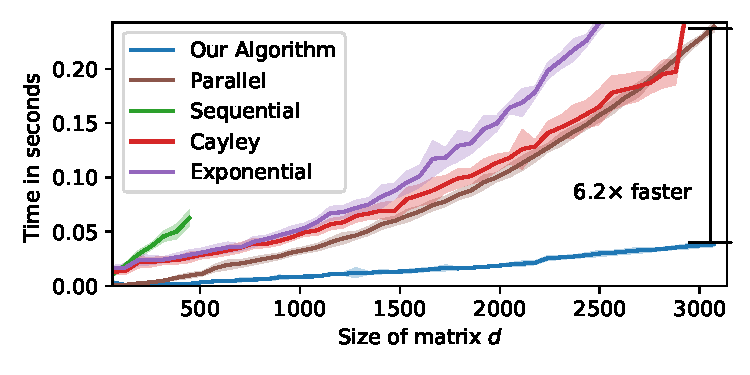
\includegraphics[width=\textwidth]{running_time}
			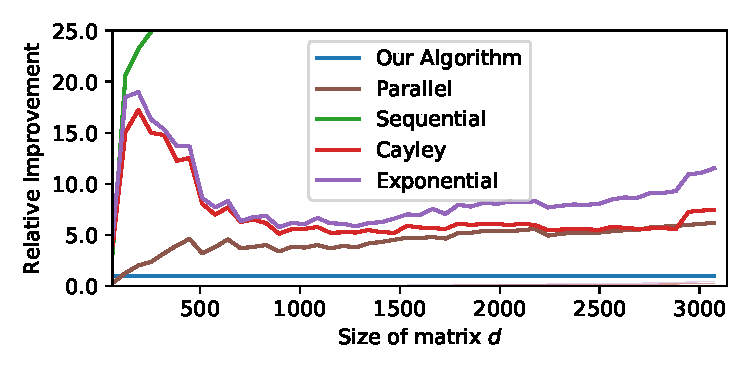
\includegraphics[width=\textwidth]{relative}
		\end{column}
	\end{columns}
\end{frame}

